% =====================================================================
%  MATH3030 Project Report
%  Build:  latexmk          (uses .latexmkrc -> XeLaTeX + biber)
% =====================================================================
\documentclass[a4paper, 11pt]{article}

% --- 1. Packages that do things (maths, figures, refs) ---------------
% =====================================================================
%  preamble.tex - functional packages only.
%  Nothing here should change how the document *looks*; that belongs in
%  themes/. Keep this file the same when you switch themes.
% =====================================================================

% --- Maths ------------------------------------------------------------
\usepackage{amsmath, amssymb, amsthm}
\usepackage{mathtools}

% --- Figures & tables -------------------------------------------------
\usepackage{graphicx}
\graphicspath{{figures/}}
\usepackage{subcaption}   % side-by-side figures: \begin{subfigure}
\usepackage{booktabs}     % nice tables: \toprule \midrule \bottomrule
\usepackage{float}
\usepackage{comment}      % \begin{comment} ... \end{comment} to hide blocks

% --- Bibliography -----------------------------------------------------
\usepackage[style=authoryear, backend=biber, maxcitenames=2]{biblatex}
%  Use \textcite{turing1952} -> "Turing (1952)"
%      \parencite{turk1991}  -> "(Turk 1991)"

% --- Links & cross-references (load hyperref late, cleveref last) -----
\usepackage{hyperref}
\usepackage[capitalise, noabbrev]{cleveref}
%  Use \cref{eq:gray-scott} -> "Equation 1", \cref{fig:spots} -> "Figure 2"

% --- Equation numbering by section: (2.1), (2.2), ... ------------------
\numberwithin{equation}{section}

% --- Theorem-like environments ----------------------------------------
\theoremstyle{definition}
\newtheorem{definition}{Definition}[section]
\newtheorem{example}[definition]{Example}
\theoremstyle{plain}
\newtheorem{theorem}[definition]{Theorem}
\newtheorem{proposition}[definition]{Proposition}
\theoremstyle{remark}
\newtheorem*{remark}{Remark}

% --- Drafting helper: \todo{...} shows in red; disable before submitting
\usepackage{xcolor}
\newcommand{\todo}[1]{\textcolor{red}{[TODO: #1]}}
% \renewcommand{\todo}[1]{}   % <- uncomment to hide all TODOs


% --- 2. Notation shortcuts -------------------------------------------
% =====================================================================
%  macros.tex - notation shortcuts. Define a symbol once here so it is
%  consistent everywhere, and can be changed in one place.
% =====================================================================

\newcommand{\R}{\mathbb{R}}
\newcommand{\diff}{\mathop{}\!\mathrm{d}}          % upright d: \diff t
\newcommand{\pd}[2]{\frac{\partial #1}{\partial #2}} % \pd{u}{t}
\newcommand{\lap}{\nabla^2}                          % Laplacian
\newcommand{\Jac}{J}                                 % Jacobian matrix
\DeclareMathOperator{\tr}{tr}                        % trace
% \det already exists in LaTeX

% Gray-Scott parameters (change symbols here if you switch convention)
\newcommand{\GSF}{F}
\newcommand{\GSk}{k}
\newcommand{\Du}{D_u}
\newcommand{\Dv}{D_v}


% --- 3. THEME: everything about how the document LOOKS ----------------
%  To change the look, point this at a different file in themes/.
%    themes/basic.tex  - plain LaTeX defaults (current)
%    themes/serif.tex  - Georgia + tighter margins, like your project plan
% =====================================================================
%  themes/basic.tex - a plain, safe starting look.
%  A theme file controls ONLY appearance: page size/margins, fonts,
%  heading style, spacing, colours, header/footer.
%  To make a new theme: copy this file, edit it, and change the
%  \input{themes/...} line in main.tex.
% =====================================================================

% --- Page layout ------------------------------------------------------
\usepackage[margin=2.5cm]{geometry}

% --- Fonts ------------------------------------------------------------
%  Default Latin Modern (works with pdfLaTeX and XeLaTeX).

% --- Paragraphs: space between, no indent ------------------------------
\usepackage[skip=6pt plus 1pt]{parskip}

% --- Links: no coloured boxes ------------------------------------------
\hypersetup{
  colorlinks = true,
  linkcolor  = black,
  citecolor  = black,
  urlcolor   = blue!50!black,
}


% --- 4. Bibliography --------------------------------------------------
\addbibresource{references.bib}

% --- Title information -------------------------------------------------
\title{Nonlinear Dynamics in Computer Graphics:\\
       Reaction--Diffusion Systems in Procedural Generation}
\author{Ragav Srinivasan}
\date{\today}

\begin{document}

\maketitle

\begin{abstract}
	We start by ti
\end{abstract}

\section{Introduction}
\label{sec:introduction}



% Structure 
\subsection{Structure of this report}
% Describe each section in their own line:
\Cref{sec:background} gives the background on reaction--diffusion systems and the phenomena they
model. We then discuss a famous result of Alan Turing on reaction--diffusion systems, and finally
focus on a simple reaction-diffusion system called the Gray--Scott model.
\Cref{sec:simulations} is my original contribution: a stability analysis of the Gray-Scott model
and a numerical simulation of it.
\Cref{sec:conclusion} gives the conclusion and possible extensions of this project.
\section{Background}
\label{sec:background}




\subsection{Procedural Generation}
\label{sec:procedural}

Procedural generation is a broad set of techniques in computer graphics that is used to create visuals, such as pseudo-realistic textures, terrains and surfaces on the fly. It eliminates the need for an artists to manually prototype and create their own worlds, Instead, a deterministic function called \emph{noise} is used to produce the desired visuals, on the fly as the player explores. This makes it possible to build large, \emph{lifelike} landscapes with mountains, rivers and vegetation with little impact to memory. \parencite{lagae2010}.

% Examples of Procedural Geneartion

Procedural generation is based on many algorithms. In this section we study one of the most widely used algorithms: \emph{Perlin Noise}.


% TODO: cite a source for the Tron / MAGI / Academy Award facts (e.g. Perlin's NYU biography page).
Ken Perlin devised his noise function after working on the visual effects for Disney's 1982 film \emph{Tron} at Mathematical Applications Group, Inc.\ (MAGI), and published it in 1985 \parencite{perlin1985}. His discovery of technique was so pivotal to the industry that it earned him an Academy Award for Technical Achievement \parencite{nyuperlin}, and still sees widespread in modern day films and video games. \parencite{lagae2010}.

\paragraph{How Perlin noise works.}
Need to write how perlin noise works next.

\paragraph{Building textures from noise.}
A single layer of noise is smooth but bland. Natural surfaces have detail at many scales, so copies of the noise at doubled frequency and halved amplitude are added together:
\begin{equation}
	\label{eq:fbm}
	\mathrm{fBm}(\mathbf{x}) = \sum_{j=0}^{n-1} \frac{1}{2^j}\, \mathrm{noise}\!\left(2^j \mathbf{x}\right),
\end{equation}
which is known as fractal Brownian motion (\cref{fig:perlin}c). Replacing $\mathrm{noise}$ by $\lvert \mathrm{noise} \rvert$ in \cref{eq:fbm} gives a ``turbulence'' function, and feeding it into a simple formula produces a material. Perlin's classic marble, for example, is $\sin\bigl(x_1 + \mathrm{turbulence}(\mathbf{x})\bigr)$ \parencite{perlin1985}


\paragraph{Limitations.}

Textures created with Perlin Noise are random and have no structure \cite{lagae2010}. Although this approach is ideal for terrain generation, it cannot be used to generate patterns found in biology such as Coral reefs, zebra stripes, Giraffe spots, etc. For this we use a different technique found in Reaction Diffusion Systems.


\subsection{Reaction Diffusion Systems}
\label{sec:rd-systems}

% Segue to reaction-diffusion systems
This brings us to the heart of this report: \emph{reaction-diffusion systems}. These are nonlinear dynamical systems, originally from chemistry, and model changes in concentrations of several chemical substances as they react and diffuse against space and time.    \parencite{turing1952}.

\emph{Diffusion} refers to the behaviour chemical substances \textit{spreading} from regions of high concentration to low concentration and as a result the substance is uniformly distributed across a medium \cite{britannicadiffusion}. It turns out that mathematically modelling this behaviour leads to an interesting variety of pattern formation called Turing Patterns. Which will be the focus of the following \cref{sec:turing-patterns}.

The general form of a reaction--diffusion system is
\begin{equation} \label{eq:rd-general}
	\pd{\mathbf{q}}{t} = D \nabla^2 \mathbf{q} + R(\mathbf{q}),
\end{equation}

% Explain the point of a dimensionless equation
Above is a dimensionless equations wherein all the physical quantities are stripped and all the terms scaled. \parencite{strogatz}.







\subsection{Turing patterns}
\label{sec:turing-patterns}

In 1952, Towards the end of Alan Turing's Life, Turing publishes one of his most seminal contributions in the field Mathematical Biology. In his 1952 paper titled "Chemical Basis of Morphogens". Turing discovers a mechanism which describes the formation of some patterns found in nature \parencite{turing1952}. For instance, the patterns found in animal skin such as the stripes of a zebra, spots of a jaguar, the structure of our brains and the formation of coral reefs are considered to be Turing patterns \parencite{sheffieldturing}.

In the paper, Turing studies the development of an embryo and describes a system of signalling molecules called \emph{Morphogens}. The reaction and diffusion shown by these morphogens can destablize the system leading to an interesting case of pattern formation \parencite{turing1952}.  

In the following section, we will be studying Turing patterns formed by a simple model called the Gray Scott Model.

\subsection{The Gray-Scott model}
\label{sec:gray-scott}

% Describes the problem
The setup for the Gray-Scott model supposes that we have a \emph{Well mixed tank} of chemical $U$. Then the concentration of $U$. We are interested in knowing the concentration of the chemical in space and time. For this, we define a vector function $u(x, t)$  that is currently unknown. We assume that chemical $U$ has the same concentration in the spatial domain except for a small patch in the center of the tank where chemical $V$ is introduced into the system. \\
\\
In chemistry, The relationship between $U$ and $V$ is defined as \textit{Autocatalysis} where the resulting product is a reactant, as is the case with $V$ is in the reaction shown below. The relationship is akin to that of \textit{prey and predator} models.

\begin{equation*}
	\underbrace{U + 2V \to 3V}_{\text{$V$ reacts to $U$ to make more of itself}}
	\qquad
	\underbrace{V \to P}_{\text{decay}}
\end{equation*}


The second rule suggests decay for $V$ by turning into an inert product $P$ which means that it becomes a non reactive substance.


% General form of the Gray Scott Model
\begin{align*}
	\frac{\partial U}{\partial t} & = -UV^2 + D_u \nabla^2 + f(1 - U) \\
	\frac{\partial V}{\partial t} & = UV^2 + D_v \nabla^2 + (k + f)V
\end{align*}
% Explaination of the terms 
\begin{itemize}
	\item $D_u$ and $D_v$ is the diffusivity of chemicals $U$ and $V$.
	\item $U$ and $V$ are the unknown vector functions representing the concentrations of the respective chemicals in space and time.
	\item $f$ is the feed rate of chemical $U$ for $V$
	\item $k$ is the decay rate for chemical $V$.
\end{itemize}



\section{Original Contribution}
\label{sec:simulations}




\subsection{Linear Stability Analysis of the Gray Scott Model}
\label{sec:stability}

Steady states of a dynamical system are states after which point the system shows no change. We consider a small disturbance around a steady state and say the state is \textit{stable} if the disturbance dampens and the system loops back to its steady state. While an \textit{unstable} steady state is when the disturbance grows over and thus the system never returns back to it's steady state \cite{strogatz}.
To give an analogy, \cref{fig:ball-analogy} compares a ball in a hilltop vs a valley. Panel (a) is a stable state as the ball returns to it's steady state after a small nudge. Panel (b) is an example of an unstable state, the ball never returns to a steady state after a small push and finally panel (c) shows a bistable state where the ball returns to a steady state but at a different point.

\begin{figure}[htbp]
	\centering
	\begin{tikzpicture}[scale=0.9, >=Stealth]
		% --- (a) Stable: ball in a valley
		\begin{scope}
			\draw[thick] (-1.6,1.3) .. controls (-0.6,-0.6) and (0.6,-0.6) .. (1.6,1.3);
			\fill[blue!60] (0,0.1) circle (0.22);
			\draw[gray, dashed] (0.72,0.42) circle (0.22);
			\draw[->, thick, red!70!black] (0.62,0.85) to[bend right=30] (0.22,0.45);
			\node at (0,-0.9) {(a) Stable};
		\end{scope}
		% --- (b) Unstable: ball on a hilltop
		\begin{scope}[xshift=4.2cm]
			\draw[thick] (-1.6,-0.4) .. controls (-0.6,1.5) and (0.6,1.5) .. (1.6,-0.4);
			\fill[blue!60] (0,1.24) circle (0.22);
			\draw[gray, dashed] (0.4,1.17) circle (0.22);
			\draw[->, thick, red!70!black] (0.65,1.45) to[bend left=30] (1.25,0.55);
			\node at (0,-0.9) {(b) Unstable};
		\end{scope}
		% --- (c) Bistable: two valleys, a big push crosses the hill
		\begin{scope}[xshift=8.6cm]
			\draw[thick] (-2.0,1.2) .. controls (-1.6,-0.5) and (-0.9,-0.5) .. (-0.6,0.3)
			.. controls (-0.3,1.0) and (0.3,1.0) .. (0.6,0.3)
			.. controls (0.9,-0.5) and (1.6,-0.5) .. (2.0,1.2);
			\fill[blue!60] (-1.26,0.03) circle (0.22);
			\draw[gray, dashed] (1.26,0.03) circle (0.22);
			\draw[->, thick, red!70!black] (-1.0,0.5) .. controls (-0.3,1.9) and (0.3,1.9) .. (1.0,0.5);
			\node at (0,-0.9) {(c) Bistable};
		\end{scope}
	\end{tikzpicture}
	\caption{Analogy of a ball on a hilltop vs a valley (a) Ball is stationary in a valley, giving a small nudge to the ball returns it back to its stationary state (b) Nudging the ball on a hilltop, the ball never comes back to it's stationary state (c) With two valleys, a large enough push carries the ball over the hill into the other stable state.}
	\label{fig:ball-analogy}
\end{figure}

Nonlinear systems such as the Gray-Scott model are difficult to solve analytically. Therefore, I will be doing a stability analysis to find out the behaviour of the system near it's steady states. To do this, we will first linearise the system by it's Jacobian Matrix and classify by its trace and determinant.


% Why this analysis for gray scott 
In this analysis I will show how diffusion can \emph{destabilise} a uniform state and result in pattern formation. The analysis will be done twice, once by dropping the coefficients of diffusion $D_u$ and $D_v$ and then we will add them back to the system and check for whether it destabilizes the system.


\begin{equation}
	\label{eq:gs-stab}
	\begin{aligned}
		\pd{U}{t} & = \Du \lap U + \underbrace{-UV^2 + \GSF(1 - U)}_{f(U,V)},   \\
		\pd{V}{t} & = \Dv \lap V + \underbrace{UV^2 - (\GSF + \GSk)V}_{g(U,V)}.
	\end{aligned}
\end{equation}

% =====================================================================
\subsubsection*{Stability Analysis without Diffusion}

Setting $\Du = \Dv = 0$ in \cref{eq:gs-stab}, every point in space behaves in the same way. We define $\dot{U}$ and $\dot{V}$:
\begin{equation}
	\label{eq:gs-nodiff}
	\begin{aligned}
		\dot{U} & = f(U, V) = -UV^2 + F(1 - U), \\
		\dot{V} & = g(U, V) = UV^2 - (F + k)V.
	\end{aligned}
\end{equation}

\paragraph{Steady states.}
A steady state needs $f = g = 0$. Factorising, $g = V\bigl(UV - (F + k)\bigr) = 0$, so either $V = 0$ or $UV = F + k$. Setting $V = 0$ yields $U = 1$. Thus $(U, V) = (1, 0)$ is a trivial steady state of the system; the case $UV = F + k$ is treated below.

\paragraph{The Jacobian.}
The Jacobian of the system is
\begin{equation}
	\label{eq:gs-jacobian}
	J =
	\begin{pmatrix}
		\dfrac{\partial f}{\partial U} & \dfrac{\partial f}{\partial V} \\[8pt]
		\dfrac{\partial g}{\partial U} & \dfrac{\partial g}{\partial V}
	\end{pmatrix}
	=
	\begin{pmatrix}
		-V^2 - F & -2UV          \\
		V^2      & 2UV - (F + k)
	\end{pmatrix}.
\end{equation}

\paragraph{The trivial steady state.}
We classify each steady state by $p = \tr J$ and $q = \det J$: it is stable if $p < 0$ and $q > 0$, and a saddle if $q < 0$; it is a node if $p^2 - 4q > 0$ and a spiral if $p^2 - 4q < 0$ \parencite{teschl2012}. At $(1, 0)$:
\begin{equation}
	\label{eq:gs-jacobian-trivial}
	J(1, 0) =
	\begin{pmatrix}
		-F & 0        \\
		0  & -(F + k)
	\end{pmatrix},
	\qquad p = -(2F + k), \qquad q = F(F + k), \qquad p^2 - 4q = k^2 .
\end{equation}
Since $F, k > 0$, we have $p < 0$, $q > 0$ and $p^2 - 4q \geq 0$, so the trivial state is a \emph{stable node for every} $F$ and $k$. A small amount of $V$ added to a tank full of $U$ simply dies out.

\paragraph{The non-trivial steady states.}
Now take $UV = F + k$. Writing $UV^2 = (UV)V$ in $f = 0$ gives $V$ in terms of $U$; substituting back into $UV = F + k$ gives a quadratic in $U$:
\begin{equation}
	\label{eq:gs-nontrivial}
	\begin{gathered}
		V = \frac{F(1 - U)}{F + k}, \qquad
		U^2 - U + c = 0 \quad \text{with } c = \frac{(F + k)^2}{F}, \\[4pt]
		U_\pm = \frac{1}{2}\left(1 \pm \sqrt{1 - \frac{4(F + k)^2}{F}}\right), \qquad
		V_\pm = \frac{F + k}{U_\pm}.
	\end{gathered}
\end{equation}
These exist only when the term under the square root is non-negative, that is, $F \geq 4(F + k)^2$, or
\begin{equation}
	\label{eq:saddle-node}
	\GSk \leq \tfrac{1}{2}\sqrt{F} - F .
\end{equation}
On the curve $k = \tfrac12\sqrt{F} - F$ the two states merge and vanish, so it is a \emph{saddle-node bifurcation} curve. Its highest point is at $F = k = 1/16$.

\paragraph{Classifying the non-trivial states.}
Using $UV = F + k$,
\begin{equation}
	\label{eq:gs-jacobian-nontrivial}
	J(U_\pm, V_\pm) =
	\begin{pmatrix}
		-V^2 - F & -2(F + k) \\
		V^2      & F + k
	\end{pmatrix},
	\qquad p = k - V^2, \qquad q = (F + k)(V^2 - F) .
\end{equation}
From the quadratic, $(F + k)^2 = FU(1 - U)$, so $V^2 = (F + k)^2/U^2 = F(1 - U)/U$ and $V^2 - F = F(1 - 2U)/U$. Since $U_+ > \tfrac12 > U_-$:
\begin{itemize}
	\item $(U_+, V_+)$ has $q < 0$, so it is a \emph{saddle} (always unstable);
	\item $(U_-, V_-)$ has $q > 0$, so it is stable when $p < 0$, i.e.\ $V_-^2 < k$. It loses stability when $p = 0$ with $q > 0$, a \emph{Hopf bifurcation}, on the curve $V_-^2 = k$.
\end{itemize}
We call $(U_-, V_-)$ the \emph{coloured state}, since it is the uniform state containing a lot of $V$.

\paragraph{Summary.}
Inside the saddle-node curve and before the Hopf curve, the well-mixed system is \emph{bistable}: the trivial state and the coloured state are both stable, separated by the saddle $(U_+, V_+)$, just like the two valleys in \cref{fig:ball-analogy}(c). Outside the saddle-node curve, only the trivial state exists. Both curves are shown in \cref{fig:stability-map}.

\begin{figure}[htbp]
	\centering
	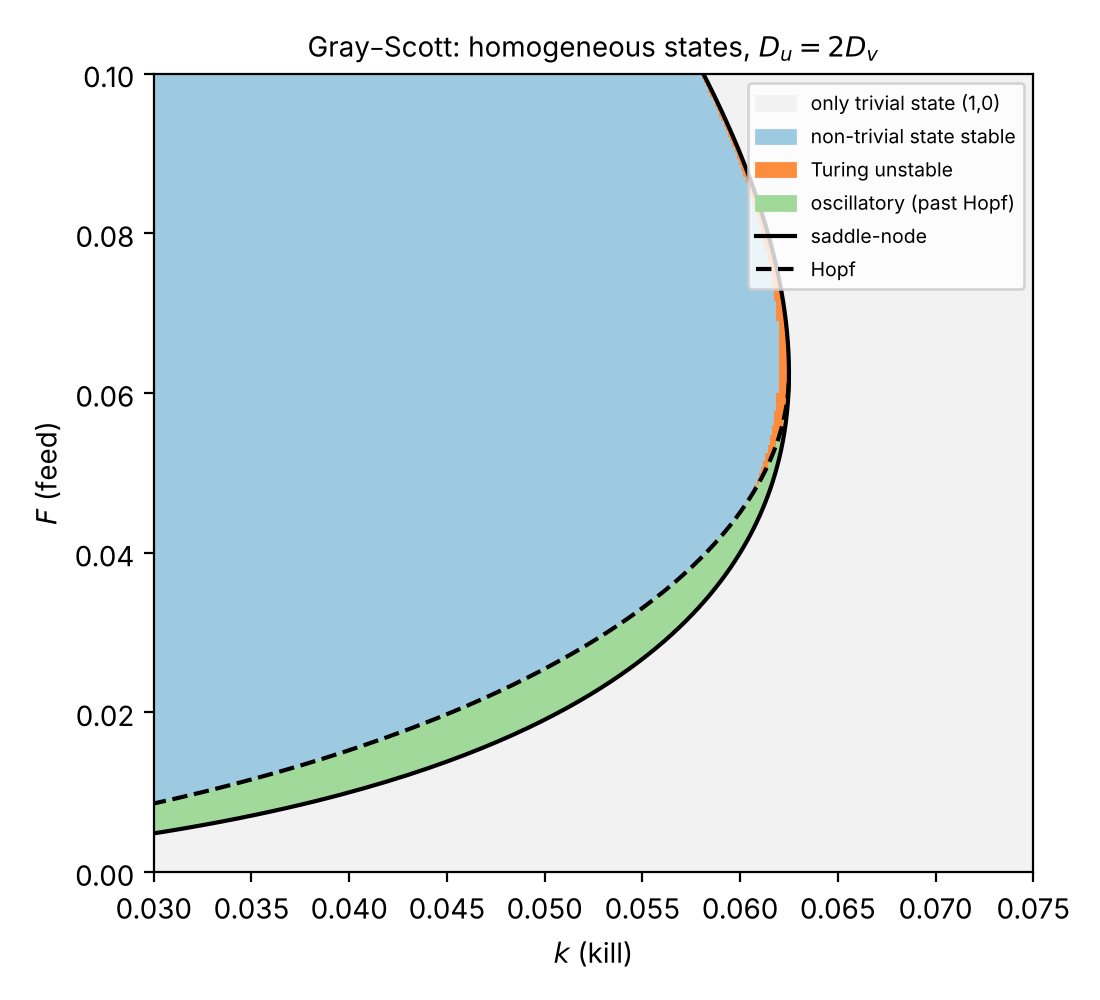
\includegraphics[width=0.65\textwidth]{stability_map.png}
	\caption{Uniform states of the Gray--Scott model with $\Du = 2\Dv$. Solid curve: saddle-node bifurcation, \cref{eq:saddle-node}. Dashed curve: Hopf bifurcation, $V_-^2 = k$. The shading shows where only the trivial state exists, where the coloured state is stable, where it is Turing unstable, and where it oscillates.}
	\label{fig:stability-map}
\end{figure}

\subsubsection*{Adding back diffusion}


\subsection{Simulation of the Gray Scott Model}
\label{sec:parameter-map}
\label{sec:numerical}
% Movtiation for doing a numerical simulation
\subsection{Texture Mapping in Blender}
\todo{I will do this section if I have time, for now I will just do the parameter map and stability analysis.}



\todo{Method details, figures and discussion.}
\section{Conclusion}
\label{sec:conclusion}
To conclude the patterns formed by Reaction Diffusion Systems and specifically the Gray Scott Model are very interesting

\printbibliography



\section{Appendix}
\end{document}

